\documentclass{beamer}
\usepackage[utf8]{inputenc}

\usetheme{Boadilla}
\usecolortheme{lily}
\usepackage{amsmath,amssymb,amsfonts,amsthm}
\usepackage{mathtools}
\usepackage{txfonts}
\usepackage{tkz-euclide}
\usepackage{listings}
\usepackage{adjustbox}
\usepackage{array}
\usepackage{tabularx}
\usepackage{lmodern}
\usepackage{circuitikz}
\usepackage{tikz}
\usepackage{graphicx}

\setbeamertemplate{footline}
{
  \leavevmode%
  \hbox{%
  \begin{beamercolorbox}[wd=\paperwidth,ht=2.25ex,dp=1ex,right]{author in head/foot}%
    \insertframenumber{} / \inserttotalframenumber\hspace*{2ex} 
  \end{beamercolorbox}}%
  \vskip0pt%
}

\usepackage{tcolorbox}
\tcbuselibrary{minted,breakable,xparse,skins}




\providecommand{\nCr}[2]{\,^{#1}C_{#2}} % nCr
\providecommand{\nPr}[2]{\,^{#1}P_{#2}} % nPr
\providecommand{\mbf}{\mathbf}
\providecommand{\pr}[1]{\ensuremath{\Pr\left(#1\right)}}
\providecommand{\qfunc}[1]{\ensuremath{Q\left(#1\right)}}
\providecommand{\sbrak}[1]{\ensuremath{{}\left[#1\right]}}
\providecommand{\lsbrak}[1]{\ensuremath{{}\left[#1\right.}}
\providecommand{\rsbrak}[1]{\ensuremath{{}\left.#1\right]}}
\providecommand{\brak}[1]{\ensuremath{\left(#1\right)}}
\providecommand{\lbrak}[1]{\ensuremath{\left(#1\right.}}
\providecommand{\rbrak}[1]{\ensuremath{\left.#1\right)}}
\providecommand{\cbrak}[1]{\ensuremath{\left\{#1\right\}}}
\providecommand{\lcbrak}[1]{\ensuremath{\left\{#1\right.}}
\providecommand{\rcbrak}[1]{\ensuremath{\left.#1\right\}}}
\theoremstyle{remark}
\newtheorem{rem}{Remark}
\newcommand{\sgn}{\mathop{\mathrm{sgn}}}
\providecommand{\abs}[1]{\left\vert#1\right\vert}
\providecommand{\res}[1]{\Res\displaylimits_{#1}} 
\providecommand{\norm}[1]{\lVert#1\rVert}
\providecommand{\mtx}[1]{\mathbf{#1}}
\providecommand{\mean}[1]{E\left[ #1 \right]}
\providecommand{\fourier}{\overset{\mathcal{F}}{ \rightleftharpoons}}
%\providecommand{\hilbert}{\overset{\mathcal{H}}{ \rightleftharpoons}}
\providecommand{\system}{\overset{\mathcal{H}}{ \longleftrightarrow}}
	%\newcommand{\solution}[2]{\textbf{Solution:}{#1}}
%\newcommand{\solution}{\noindent \textbf{Solution: }}
\providecommand{\dec}[2]{\ensuremath{\overset{#1}{\underset{#2}{\gtrless}}}}
\newcommand{\myvec}[1]{\ensuremath{\begin{pmatrix}#1\end{pmatrix}}}
\let\vec\mathbf

\lstset{
%language=C,
frame=single, 
breaklines=true,
columns=fullflexible
}

\numberwithin{equation}{section}

\lstset{
  language=Python,
  basicstyle=\ttfamily\small,
  keywordstyle=\color{blue},
  stringstyle=\color{orange},
  numbers=left,
  numberstyle=\tiny\color{gray},
  breaklines=true,
  showstringspaces=false
}

\title{Problem 5.2.26}
\author{ee25btech11023-Venkata Sai}

\date{\today} 
\begin{document}

\begin{frame}
\titlepage
\end{frame}

\section*{Outline}
\begin{frame}
\tableofcontents
\end{frame}

\section{Problem}

\begin{frame}
\frametitle{Problem}
\setcounter{section}{1}
Slope of a line passing through $\vec{P}\brak{2,3}$ and intersecting the line $x+y=7$ at a distance of 4 units from $\vec{P}$, is
\end{frame}
%\subsection{Literature}
\section{Solution}

\subsection{Matrix Equation}
\begin{frame}
\frametitle{Matrix Equation}
Given  
\begin{align}
\frac{x}{a}-\frac{y}{b}=0 \implies bx-ay=0 \\
ax+by=a^{2}+b^{2} 
\end{align}
The matrix equation for a line is defined as
\begin{align}
    \vec{n}^\top\vec{x}=c
\end{align}
where $\vec{n}$ is the coefficient matrix and $\vec{x}=\myvec{x\\y}$
\begin{align}
    \myvec{b&-a}\vec{x}=0
    \end{align}
    \begin{align}
    \myvec{a&b}\vec{x}=a^{2}+b^{2} 
\end{align}
As a matrix equation
\begin{align}
 \myvec{b&-a\\a&b}\vec{x}=\myvec{0\\a^{2}+b^{2}} 
  \end{align}
\end{frame}
\subsection{Transpose}
\begin{frame}
\frametitle{Transpose}
 \begin{align}
    \myvec{b&-a\\a&b}^\top\myvec{b&-a\\a&b}\vec{x}= \myvec{b&-a\\a&b}^\top\myvec{0\\a^{2}+b^{2}} 
    \end{align}
       \begin{align}
    \myvec{b&a\\-a&b}\myvec{b&-a\\a&b}\vec{x}= \myvec{b&a\\-a&b}\myvec{0\\a^{2}+b^{2}}  
  \end{align}
  \begin{align}
\myvec{a^{2}+b^{2}&0\\0&a^{2}+b^{2}}\vec{x}=\myvec{a\brak{a^{2}+b^{2}}\\b\brak{a^{2}+b^{2}}}
  \end{align}
  \begin{align}
\brak{a^{2}+b^{2}}\vec{I}\vec{x}=\myvec{a\brak{a^{2}+b^{2}}\\b\brak{a^{2}+b^{2}}} 
\end{align}
\begin{align}
\vec{I}\vec{x}=\myvec{a\brak{a^{2}+b^{2}}\\b\brak{a^{2}+b^{2}}} \frac{1}{a^{2}+b^{2}} 
  \end{align}
\end{frame}
\begin{frame}
\subsection{Conclusion}
\frametitle{Conclusion}
 \begin{align}
      \vec{I}\vec{x}=\myvec{a\\b}
  \end{align}
  \begin{align}
      \myvec{x\\y}=\myvec{a\\b}
  \end{align}
  Hence $x=a,y=b$ is the solution for given system of linear equations
\end{frame}
\subsection{Plot}
\begin{frame}[fragile]
\frametitle{Plot}

\begin{figure}[h!]
   \centering
   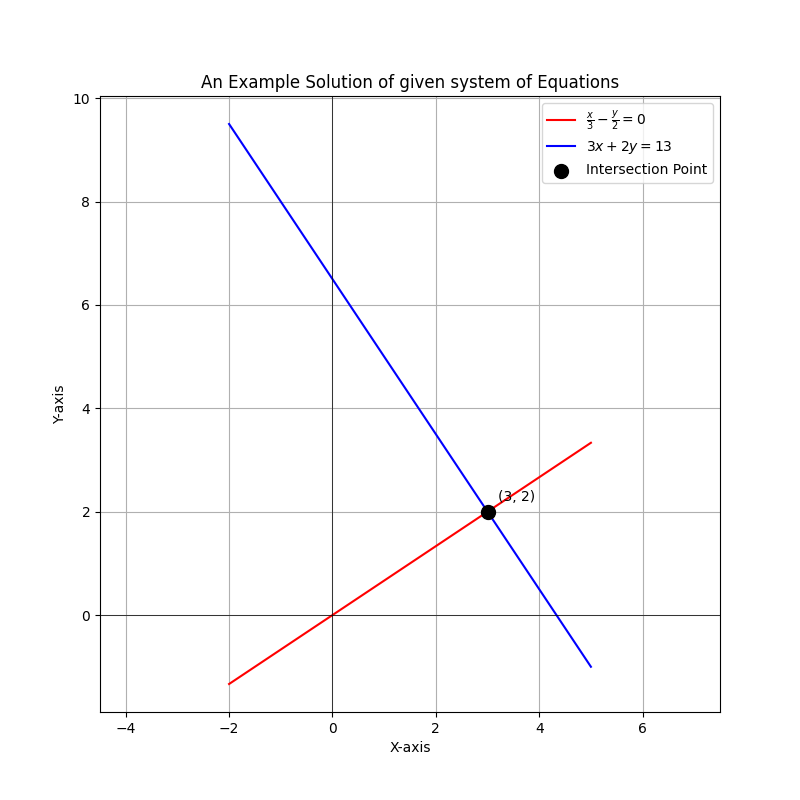
\includegraphics[width=0.7\columnwidth]{figs/fig1.png}
	\caption{}
   \label{}
\end{figure}
\end{frame}

\section{C Code}
\begin{frame}[fragile]
\frametitle{C Code}
\begin{lstlisting}[language=C]
void get_system_coeffs(double* out_coeffs) {
 
    double a = 3.0;
    double b = 2.0;
   
    out_coeffs[0] = b;
    out_coeffs[1] = -a;
    out_coeffs[2] = a;
    out_coeffs[3] = b;
 
    out_coeffs[4] = 0;
    out_coeffs[5] = a*a + b*b;
 
    out_coeffs[6] = a;
    out_coeffs[7] = b;
}
    \end{lstlisting}
\end{frame}
\section{Python Code}
\begin{frame}[fragile]
\frametitle{Python Code for Calling}
\begin{lstlisting}[language=Python]
import ctypes
import numpy as np
from sympy import Matrix  

def solve_and_prepare_data():
    
    lib = ctypes.CDLL('./code.so')
    double_array_8 = ctypes.c_double * 8
    lib.get_system_coeffs.argtypes = [ctypes.POINTER(ctypes.c_double)]
    out_data_c = double_array_8()
    lib.get_system_coeffs(out_data_c)
    raw_data = list(out_data_c)
    
    # Unpack the raw data
    m_coeffs = raw_data[0:4]
    c_coeffs = raw_data[4:6]
    a, b = raw_data[6], raw_data[7]
\end{lstlisting}
\end{frame}
\begin{frame}[fragile]
\frametitle{Python Code for Solving}
\begin{lstlisting}[language=Python]
    aug_M = Matrix([
        [m_coeffs[0], m_coeffs[1], c_coeffs[0]],
        [m_coeffs[2], m_coeffs[3], c_coeffs[1]]
    ])
    rref_matrix, _ = aug_M.rref()
    solution_P = np.array(rref_matrix[:, -1]).astype(np.float64).flatten()
    x_start, x_end = -2.0, a + 2.0
    y1_start, y1_end = (b/a) * x_start, (b/a) * x_end
    y2_start, y2_end = (-a/b) * x_start + (a**2 + b**2)/b, (-a/b) * x_end + (a**2 + b**2)/b
  
    return {
        "line1_x": [x_start, x_end], "line1_y": [y1_start, y1_end],
        "line2_x": [x_start, x_end], "line2_y": [y2_start, y2_end],
        "solution_point": solution_P,
        "a": a, "b": b
    }
\end{lstlisting}
\end{frame}
\begin{frame}[fragile]
\frametitle{Python Code for Plotting}
\begin{lstlisting}[language=Python]
#Code by GVV Sharma
#September 12, 2023
#Revised July 21, 2024
#released under GNU GPL
import sys                                          #for path to external scripts
sys.path.insert(0, '/workspaces/urban-potato/matgeo/codes/CoordGeo/') 
import matplotlib.pyplot as plt
import numpy as np
from call import solve_and_prepare_data

plot_data = solve_and_prepare_data()

line1_x = plot_data["line1_x"]
line1_y = plot_data["line1_y"]
line2_x = plot_data["line2_x"]
line2_y = plot_data["line2_y"]
x_sol, y_sol = plot_data["solution_point"]
a, b = plot_data["a"], plot_data["b"]

\end{lstlisting}
\end{frame}
\begin{frame}[fragile]
\frametitle{Python Code for Plotting}
\begin{lstlisting}[language=Python]
print(f"Plotting solution for a={a:.0f}, b={b:.0f}: Point is ({x_sol:.0f}, {y_sol:.0f})")

fig, ax = plt.subplots(figsize=(8, 8))

# Use the unpacked lists directly
ax.plot(line1_x, line1_y, 'r-', label=f'$\\frac{{x}}{{{a:.0f}}} - \\frac{{y}}{{{b:.0f}}} = 0$')
ax.plot(line2_x, line2_y, 'b-', label=f'${a:.0f}x + {b:.0f}y = {a**2 + b**2:.0f}$')
ax.scatter(x_sol, y_sol, color='black', s=100, zorder=5, label='Intersection Point')
ax.text(x_sol + 0.2, y_sol + 0.2, f'({x_sol:.0f}, {y_sol:.0f})')

ax.set_title('An Example Solution of given system of Equations')
ax.set_xlabel('X-axis')
ax.set_ylabel('Y-axis')
\end{lstlisting}
\end{frame}

\begin{frame}[fragile]
\frametitle{Python Code for Plotting}
\begin{lstlisting}[language=Python] 
ax.grid(True)
ax.axhline(0, color='k', linewidth=0.5)
ax.axvline(0, color='k', linewidth=0.5)
ax.axis('equal')
ax.legend()
plt.show()
plt.savefig('fig1.png')
\end{lstlisting}
\end{frame}

\end{document}